\documentclass[journal]{vgtc}                % final (journal style)
%\documentclass[review, journal]{vgtc}         % review (journal style)
%\documentclass[widereview]{vgtc}             % wide-spaced review
%\documentclass[preprint, journal]{vgtc}       % preprint (journal style)
%\documentclass[electronic, journal]{vgtc}     % electronic version, journal

%% Uncomment one of the lines above depending on where your paper is
%% in the conference process. ``review'' and ``widereview'' are for review
%% submission, ``preprint'' is for pre-publication, and the final version
%% doesn't use a specific qualifier. Further, ``electronic'' includes
%% hyper-references for more convenient online viewing.

%% Please use one of the ``review'' options in combination with the
%% assigned online id (see below) ONLY if your paper uses a double blind
%% review process. Some conferences, like IEEE Vis and InfoVis, have NOT
%% in the past.

%% Please note that the use of figures other than the optional teaser, is not permitted on the first page
%% of the journal version.  Figures should begin on the second page and be
%% in CMYK or Grey scale format, otherwise, colour shifting may occur
%% during the printing process.  Papers submitted with figures other than the optional teaser on the
%% first page will be refused.

%% These three lines bring in essential packages: ``mathptmx'' for Type 1
%% typefaces, ``graphicx'' for inclusion of EPS figures. and ``times''
%% for proper handling of the times font family.

\usepackage{mathptmx}
\usepackage{graphicx}
\usepackage{times}
\usepackage{float}

%% We encourage the use of mathptmx for consistent usage of times font
%% throughout the proceedings. However, if, you encounter conflicts
%% with other math-related packages, you may want to disable it.

%% This turns references into clickable hyperlinks.
\usepackage[bookmarks,backref=true,linkcolor=black]{hyperref} %,colorlinks
\hypersetup{
  pdfauthor = {},
  pdftitle = {},
  pdfsubject = {},
  pdfkeywords = {},
  colorlinks=true,
  linkcolor= black,
  citecolor= black,
  pageanchor=true,
  urlcolor = black,
  plainpages = false,
  linktocpage
}

%% If you are submitting a paper to a conference for review with a double
%% blind reviewing process, please replace the value ``0'' below with your
%% OnlineID. Otherwise, you may safely leave it at ``0''.
\onlineid{0}

%% declare the category of your paper, only shown in review mode
\vgtccategory{Research}

%% allow for this line if you want the electronic option to work properly
\vgtcinsertpkg

%% In preprint mode you may define your own headline.
%\preprinttext{To appear in an IEEE VGTC sponsored conference.}

%% Paper title.

\title{Visually Explaining the Weight Distribution of Neural Networks Over Time}
%canwe make it Developments instead of distribution

%% This is how authors are specified in the journal style

%% indicate IEEE Member or Student Member in form indicated below
\author{Sahil Pasricha\\\textit{Advisor 1:} Thilo Spinner\\\textit{Advisor 2:} Hanna Sch{\"a}fer\\\textit{Supervisor:} Daniel A. Keim}

\authorfooter{
\item[]
Sahil Pasricha, Thilo Spinner, Hanna Sch{\"a}fer, and Daniel A. Keim are with the University of Konstanz.\\
\item[]
E-mail: \{sahil.pasricha, thilo.spinner, hanna.schaefer, keim\}@uni-konstanz.de.
}

%other entries to be set up for journal
%\shortauthortitle{Biv \MakeLowercase{\textit{et al.}}: Global Illumination for Fun and Profit}
%\shortauthortitle{Firstauthor \MakeLowercase{\textit{et al.}}: Paper Title}

%% ABSTRACT
\abstract{We present an interactive visualization method of the statistical distribution of weight over learning steps.
A representation that assists the user with insights about the ML process, expediting model optimization procedure with measured calculations to improve the accuracy of a model.
This visualization assists the user to understand the quality of the model and leverage the insights to further optimize the ML algorithm.
We investigate the design space of explanation processes based on core factors of machine learning algorithms to present the learning process using the distribution of weights over the time steps.
To support this, we analyse visualization parameters and summary statistics to present the data in a condensed form without compromising the potentially critical information in context.
Specifically, we examine complex time series, clustering and sorting methods. Based on the learning derived from our analysis,
we introduce distinctive combinations of Central Data Tendency with ML algorithms to present different perspectives for data exploration. Furthermore, to demonstrate the utility of the method, we evaluate our method with different models and data sets to observe interesting patterns. The most
interesting insights that our method presented, comes from a model with bad accuracy. By observing the visualization, we analyse that the model finds perfect weights which represent train data and this happens in very initial training steps. In conclusion, this model requires more training data to optimize accuracy.} % end of abstract

%% Keywords that describe your work. Will show as 'Index Terms' in journal
%% please capitalize first letter and insert punctuation after last keyword
\keywords{ Visualization, Interactive Machine Learning (IML), Deep Neural Networks (DNN), Explainable AI, Visual Analytics, Interpretability, Explainability, Central Data Tendency (CDT), Dynamic Time Warping, Time Series Analysis}

%% ACM Computing Classification System (CCS). 
%% See <http://www.acm.org/class/1998/> for details.
%% The ``\CCScat'' command takes four arguments.

\CCScatlist{ % not used in journal version
 \CCScat{K.6.1}{Management of Computing and Information Systems}%
{Project and People Management}{Life Cycle};
 \CCScat{K.7.m}{The Computing Profession}{Miscellaneous}{Ethics}
}

%% Uncomment below to include a teaser figure.
\teaser{
 \centering
 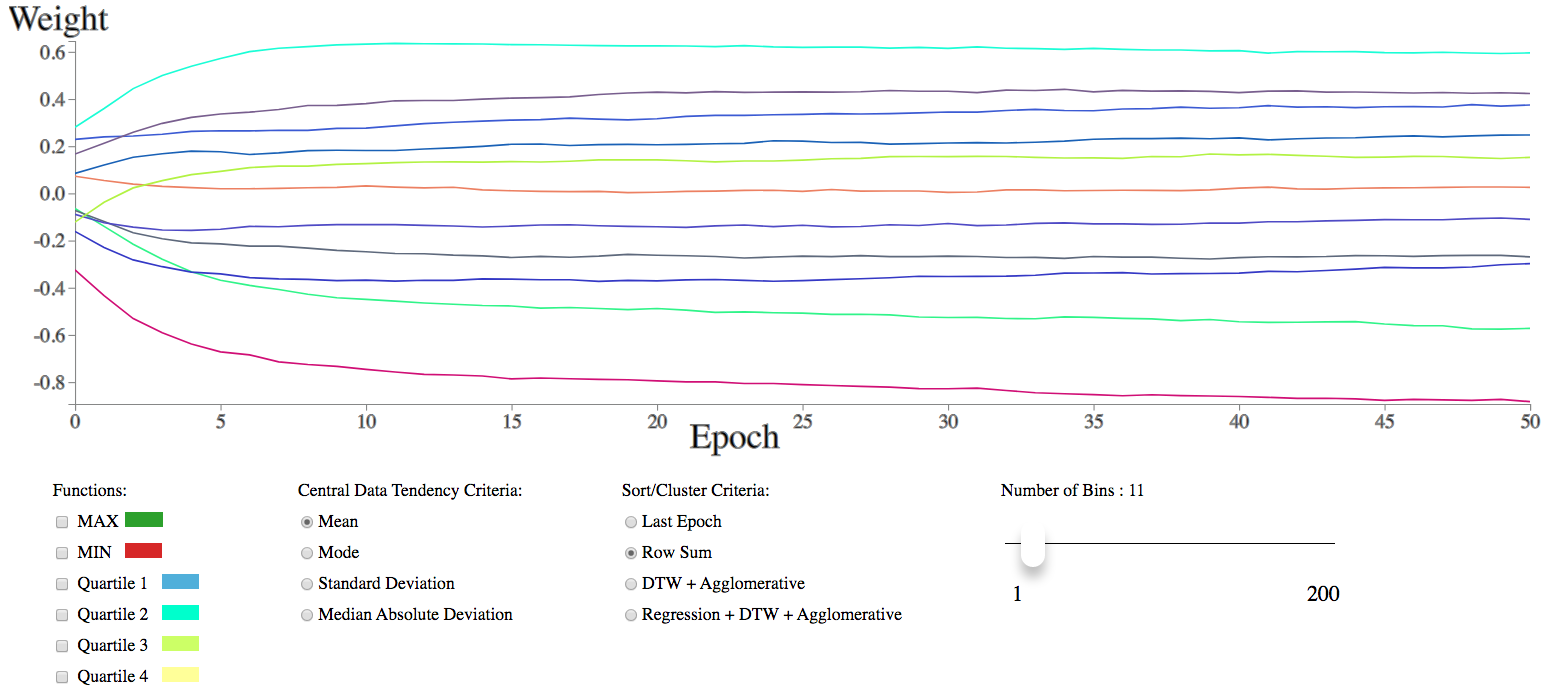
\includegraphics[width=12cm]{teasered.png}
 \caption{A summarized view of features offered by the proposed visualization method. The pattern indicates a higher degree of learning in initial training steps as compared to later steps.}
 \label{teaser}
}

%% Uncomment below to disable the manuscript note
\renewcommand{\manuscriptnotetxt}{}

%% Copyright space is enabled by default as required by guidelines.
%% It is disabled by the 'review' option or via the following command:
% \nocopyrightspace

%%%%%%%%%%%%%%%%%%%%%%%%%%%%%%%%%%%%%%%%%%%%%%%%%%%%%%%%%%%%%%%%
%%%%%%%%%%%%%%%%%%%%%% START OF THE PAPER %%%%%%%%%%%%%%%%%%%%%%
%%%%%%%%%%%%%%%%%%%%%%%%%%%%%%%%%%%%%%%%%%%%%%%%%%%%%%%%%%%%%%%%%

\begin{document}

%% The ``\maketitle'' command must be the first command after the
%% ``\begin{document}'' command. It prepares and prints the title block.

%% the only exception to this rule is the \firstsection command


\maketitle

%% \section{Introduction} %for journal use above \firstsection{..} instead

\section{Motivation} %(Motivation, Problem Description, Contributions)
With technology touching our life closer than ever before we have become heavily dependent on machine made decisions.
We use it for varied tasks ranging from recognizing our face over unlocking smartphone to landing a 70 ton aircraft. Along with the growth in the frequency of AI being used in everyday life, the role of these machine made decisions have witnessed a surge in recent times. Given that, popular AI systems have already achieved considerable accuracy, what makes it susceptible is its inability to explain decisions it didn't make right.

Presently in a typical scenario, users apply a random algorithm for machine learning and iterate the process until it reaches desirable accuracy \cite{blackbox}. The fact is, this black box methodology works quite often but not always. But the majority of applications of AI are not mission critical and those which are, have already started working on Explainable Artificial Intelligence (XAI) to further dig into the model to understand its core. This application mainly includes autonomous driving, satellite imaging and autopilot for drones \cite{darpa}.

Speaking of XAI, 
modern deep learning platforms including 
TensorFlow \cite{tensorflow} provide libraries to generate a low-level dataflow chart that supports a diversity of learning algorithms.
While these graphs can be suitable for
models that are typically small  but as the
size grows, these dataflow graphs present
thousands of complex, low-level operations
that may overwhelm the user with too much information.

Apart from these conventional tools, there has been considerable progress in the direction of customized XAI methods
that take the explanations to various degrees and directions ranging from
explaining the feature importance by visual maps (saliency maps) \cite{saliency} for explaining individual prediction (LIME) \cite{lime}.
The recent research over interactive and Explainable Machine Learning \cite{xai} \cite{xai2} provides an entry point to classifications of
existing XAI methods.
Also, a survey paper \cite{2019survey} sheds light on the interpretability of these models.
Something common in almost all of the existing XAI models is the dependency and integration.
All of them are designed to work with a definite domain, data or model and
do not offer plug and play implementation with active ML developing and debugging process.
None of them seem to be designed for an ML expert who typically works on ML models from varied domains, has different structures, and trains on diverse data sets. 

This motivates us to research in the direction of a 
domain, data and model independent
XAI method
that facilitates an ML expert with ML algorithm's quality analysis
through a visual exploration of its learning process, whose patterns
may further reveal additional interesting insights.
In addition, we not only want to describe the theoretical workflow but also deliver system implementation.
Because the foundation of our proposed model are core feature of
almost every ML algorithm, it is comparatively quick to implement.
Our visualization method provides an interactive analysis of the learning process of an ML model.

This design study\cite{designStudy} began with evaluating fundamental features to determine the critical insights they could offer about the model.  The next step was to research methods to present that in summarized and meaningful ways without information loss, this included 
evaluating basic methods like mean, median for central data tendency and
introduced novel combination of sorting, clustering and time series algorithms to form bins/clusters that have more homogeneous data. 
To support exploration, we employed interactive zoom, log scale,
 adaptive binning and flexibility over bin count.
Finally, 
we evaluated the usability of our method on specific data sets and analyzed
how the revealed patterns can support a user in establishing a hypothesis about the quality of the model and explore possible ways to enhance the accuracy of the model through rich interactions.

\section{Related Work}
To devise a novel XAI method, we analyse existing research
on XAI models, Information Visualization and
survey papers that compared XAI methods on multiple scales.
We also studied research analysing the impact of perturbation weights of an NN model \cite{microsoft2015modeltracker}.

We start with understanding the features and scope of existing XAI models\cite{mein}. 
Information flow \cite{infomationflow} is one such method offering an overview of dataflow between groups of operations exhibiting
details of its nested structure on demand. 
In contrast, LIME \cite{lime}  focus solely upon explaining features
and ANCHORS \cite{anchors}  uses novel  model-agnostic 
explanations based on if-then rules, 
called anchors.
 By visualizing model  performance while  enabling  direct  data  inspection, model tracker \cite{microsoft2015modeltracker} offer direct
error examination and debugging empowering user with useful controls right from GUI.
Another technique called Layer-wise Relevance Propagation  \cite{LRP} explains the model’s outcomes by decomposition. 
It reverse-engineers the output using local redistribution rules until it assigns a relevance score.
Survey papers  \cite{xai,2019survey} were critical to understand the dependency of these models.
All of these models have used complex methods to derive
important insights from the model by pondering upon the usability of any aspect of the model (weights, layers, structure) by harnessing its relation to other aspects and impact on output. This also inspire us to experiment methods (discussed in later section) that are novel to XAI methods.

To further broaden our knowledge on usage of visual analytics to understand the concepts of \cite{IMLViz} to Hierarchical topic analysis and visual pattern mining. Novel parameters were introduced by explAIner \cite{xai} to classify XAI models \cite{xai3}. 

We also find some existing research that sheds light on the effects of input and weight perturbations of the output on a neural network \cite{sensitivity}. This paper also suggests an explanation to express a relation between neurons output errors and its input and weight errors.


\section{Problem Characterisation}
One feature common in every ML model is the enormous size.
Optimizing these models further needs a complete understanding of intrinsic features.
While we have methods to visualize ML models, most of them either represent only the higher-level picture and others offer detailed information but on local levels or outputs \cite{xai3}.
At times, these explanation methods need to be mapped to the features of a given domain, post which they are fragile to change in data, domain or model. 
Moreover, if an ML expert who works on multiple models from varied domain wants to get some insights about his model, the time required to implement existing visualization models makes it far more impractical to use them. 
Even if we consider that they are implemented in no time, all of those models work on a feature level and may overwhelm the user by presenting granular details.
To create a method that can be useful for a broad application range,
we can use something very generic that highlights crucial information about the model. This guides us to think of weights,
as their development over time reveals a model's learning patterns which may further point to interesting insights.
Even though weights looks promising to proceed with, it comes with complexities of huge data size and number of variables.

The fact that values are both positive and negative makes it complex to apply methods like binning due to possibility of oppositely signed values neutralizing each other. 
While most of the existing research is directed towards external features to explain the model, there is also a possibility of deriving insights from intrinsic features. Sighting the research gap between the aforementioned methods, we proceed with our research towards exploring the solutions towards possible usability of fundamental features.

\begin{figure}
    \includegraphics[width=8.5cm,height=5cm] {Images/log_scale.png}
    \caption{A combination of log scale and interactive brush applied on figure \ref{teaser}. This directs the focus towards specific epochs and present detailed view by assigning more space to weights near zero}
    \label{fig:log_scale}
\end{figure}

\section{Choosing feature to explain   }%needs , problems and requirements
We begin by explaining that the target here is to make the user get insights about the ML model\cite{mein}
that can assist him to assimilate the learning and point out the possible reasons for bad accuracy. A bigger challenge is doing all this irrespective of the kind of data, domain or model. Likewise, for the same reasons, we are assuming our end user to be an expert in ML applications with a sound understanding of mathematics.

While many other researchers have tried to solve this seemingly easier problem, the crux of the problem lies in the fact that any ML model requires domain knowledge to understand the features and results. Now, when researchers try explaining these outputs, they ended up tailoring the system to fit the domain needs. This, on one side had a great advantage as that particular given domain got its explanations right and hence an output can be explained to a considerable extent while, on the other hand, the solution was useful for that domain only and will need constant updating. Some examples of such models are LIME\cite{lime} and ANCHORS\cite{anchors} this make us realize the fact that despite putting efforts, the usability of any explanation gets limited to the data, model and domain that it supports.
Thinking this, we intensify our research in directions of developing a solution that supports the needs of diverse domains rather then just specializing for one. However, this seemed implausible at the application level which directs our path towards the fundamentals of ML decision making and focused our attention on data, model, weights, bias, activation function, inputs layer, output layer, etc. While they all seem useful for research in XAI, we narrow our focus based on bias and weights to be most useful for the explanation as they impact the model at minuscule levels. Among these two, weights proved more informative in finding fractions of the model that were learning, segments of the model that were contributing to the outputs to a higher degree along with the point in learning steps where model stops to learn. We realized that further study of weights can even help us find out the parts of the model that we can prune with least impact on accuracy. The last point seems absurd in a world where we are constantly thriving for accuracy but then there are also scenarios where an ML algorithm can not be applied only because the processing power it needs is just not feasible ,affordable or available in today's world.

%why weight pruning needs balanced information
% Making the network enough vast to fit a mantle map.  In the absence of a complete perspective, users have to make decisions with limited insights 


\section{Model, Data Set and Data Abstraction}
%Visual encoding  and Interaction

In this section, we define the progress from choosing features to design through an iterative pipeline.
Starting with selecting data set for analysis during research and
checking appropriate models. Followed by analysing features and statistics for data abstraction.

Before proceeding to visualization we would like to introduce the data sets we use in our analysis.
These constitute MNIST\cite{mnist}, Cifar10\cite{cifar10} and Twitter airlines review data sets\cite{airlines} with CNN and dense models for analysis.
As we progressed through various methods for visualisations , we analysed each of them on data sets and models mentioned above.
For the sake of comparison,  all the figures mentioned till section 6.5 are created using same input i.e MNIST data set and Dense model.
This model demonstrated a sharp increase in accuracy for initial epochs (Detailed statistics about accuracy and loss are shared in appendix).

We then develop a python script to print weights during the training process and store them in a .csv file.
These csv file store 2 dimension data (Training step, n dimension feature vector) of weight distribution during learning.
We also plan to check our visualization on data with a varied loss, hence we altered our models to generate results with range of loss.
This includes the addition of an extra layer, changing the number of units in layers, 
using different activation functions and updating the learning rate. 
% why we need to summarize data 
For a small ML model with 2 layers and 50 Ids in each,  training on MNIST data set will have approx 40,000 individual weights on any given training step. Representing all these weights individually will
choke any visualization and may render it useless, while abstracting data may result in loss of information by averaging out the weight fluctuation of individual Id in group.

Basic methods like mean and median that are easy to apply and explain,
what makes the choice difficult is the trade-off between abstraction and loss of information.
Moreover, weights being both positive and negative makes the grouping of data a critical operation and needs detailed analysis explained in next section.
\begin{figure}
    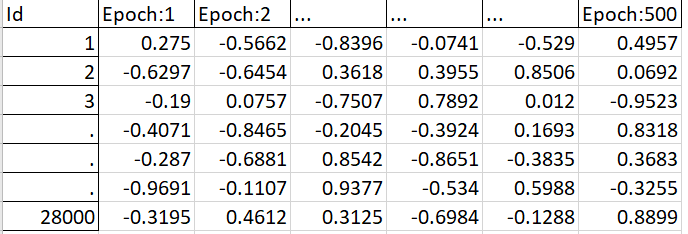
\includegraphics[scale =0.7] {sample_data.png}
    \caption{A typical csv of model weights. Rows denote Ids/feature vector and columns depict how their values change over training steps/Epoch.}
    \label{fig:csv}
\end{figure}

\section{Visualization Design and Strategy  }
For visualization design, we start with analysing complex visualization
including hierarchical edge bundling, node-link tree and radial cluster layout
that suit initial needs of research. However, as our study progressed
towards complex methods like DTW (explained later) and clustering, we direct our focus to
a relatively simple visualization.
Multi-line chart suits best here for it is simple to be understood and gives the user the ability to focus on understanding the complex methods as well as the leanings that these patterns symbolize.  
Next, we planned on designing a strategy to make our visualization interactive, flexible and scalable. Therefore, we devise a plan of methods and methodologies that encompass our visualization. The goal of having the strategy is simply to make the user understand the distribution of weights during the training process which she/he can further use to form a hypothesis. This primarily includes: 
\begin{itemize}
\item Interactive zoom - We are operating with complex models, It is certain to receive data which can not be presented along with the details on one screen. On the other hand, omitting a local view may abstain the user from noticing the details at granular levels in the model. We choose to deploy interactive zoom over training steps. This feature zoom in to the selected interval on y-axis using brush pattern. 
\item Flexibility over the number of bins - User can select the size based on the level of detail she/he is searching for.
\item Model States - We are collecting weights throughout the training process and representing changes in data over training steps which makes single model state as best suited explanation strategy in our case 
\item Visualization scope - To build a visualization based on intrinsic features, is most important to select a model-only visualization which primarily aims at presenting the fundamentals rather than explaining outputs  \cite{verbalization}
\item Log scale - Its useful to display numerical data over a very wide range of values in a compact way by assigning more spatial space to values nearby zero.
\end{itemize}
Once through with these, the next big step is summarizing the data. 
To avail easy comparison with the focus on representing a large amount of information as simply as possible, we used the following aspects of summary statistics.

% inform that we are using line graph 
\subsection{Central Data Tendency}This includes statistically calculating the tendency of data to cluster around a middle value \cite{cdt}. In our context, this measure is used for summarizing the data to present it to the user for visual exploration. It starts with a simple logic of using the mean to represent a rather larger data set. Though it looks simple, but forms the most complex part of our project which requires an extensive research. Major reason for the same is that we want to present a wide data range using single visualization with least loss of information. For the same purpose, we start evaluating relatively easy methods and progress further.

\subsubsection{Mean of all training steps} Though it gives a viable view of Central Data Tendency (CDT),  but it completely blankets the visualization of the learning process as all the training steps are now combined into one. Thus rendering it an implausible option.

\subsubsection{Mean of all Ids} It has an advantage of not compromising the training process visualization, yet it comes with its own limitations that includes: 

\begin{itemize}
\item Negative and positive weighs neutralizing each other.
\item All Ids being combined to one thereby hiding the lower level details.
			As seen in figure.\ref{fig:mean_all_in_1} , all the Ids are represented by single line. 
While both of the above mentioned problems looked dissimilar, their solutions i.e. sorting and binning (as we will study later in this section) are interconnected. 
\end{itemize}
\begin{figure}
    \includegraphics[width=8.5cm,height=5cm] {Images/mean.png}
    \caption{A line chart representing the development of weights over training steps/epochs. Here, all Ids are represented as a single line using mean.}
    \label{fig:mean_all_in_1}
\end{figure}


\subsubsection{Mode}It can turn useful to inform the user about the most occurred value at a given training step. But, this has its own limitations :
\begin{itemize}
\item It tells the user most occurred item, but not the frequency of its occurrences.
\item It may miss outliers.
On the contrary, it has one positive point over mean, i.e. there is no chance of positive and negative weights averaging each other
While the above factors prove that mode may not be the best indicator of CDT, we will  use mode at some later point just to add a different visualization to the user which may prove helpful in many cases. 
\end{itemize}

\subsection{Binning }
We use binning to make bins to group the adjacent/similar weights together. This helps the user understand the intermediate picture between the mean ( all data presented using a single line on a line chart ) and every individual Id presented by a line (the chart becomes obsolete as soon as the number of Ids exceeds 100, which it does in most cases).
As discussed already, binning possesses a huge challenge as it may put weights with different signs in the same group and they end up averaging each other out. Furthermore, in binning, we considered evaluating the following options: 

Equal Width Binning - Though it easy to understand, the idea for using it is discarded as weights are highly dynamic and their range may drastically differ from one model/data to another. Fixing width/weight intervals may prove obsolete and ineffective.
% add an image?

Equal Depth Binning - This is also discarded from being used without much consideration because we notice that much of the weights exists within range of -0.5 to +0.5 and this binning  makes bigger bins around the range boundaries, which again, may not be very helpful to understand the weight distributions.
% add an image?

Adaptive Binning\cite{binning}. The main purpose of this is to have dynamic X and Y-axis intervals to support any given range of data.
Here we decide to bin the Ids as we study the limitation of "mean by Ids" we know exactly that we need flexibility over the number of bins size and hence over data abstraction and visualization. 
Moreover, flexibility in the number of bins may offer a visualization that can reveal interesting patterns as bin sizes vary with the bin count.
Hence, we decide to use a scroll bar scaled from 1 to 200  to decide on the number of bins needed. Value one gives a visualization of maximum compressed (mean of all Ids) data while as user increase the number of bins, the data compression eases and one can see a more in-depth view. For instance, in a NN where we have 100 Epochs and 200 Ids, when you make bin count to 1, the chart displays single line i.e mean of 200 Ids at any given epoch. Now, when you set the same scroll bar value to 20, the number of bins increases to 20 and bin size is now 200/20 i.e 10, one line on the chart is now presenting the summarized view of 10 Ids rather than 200 which offer more clearer and less generalized visualizations that are closer to individual weights.

This also has a flaw, as the bins were just made out of adjacent Ids with no order of weights. Hence either negative and positive weights may even each other out, making the output unsubstantiated. This directs us further in the direction of our next step i.e Sorting method.


\begin{figure}
    \includegraphics[width=8.5cm,height=5.5cm]{Images/sorting/first_epoch.png}
    \caption{Sorting weights in ascending order of values at first epoch. The straight lines are due to +ve and -ve weights averaging each other within a bin.}
    \label{fig:sort_first_epoch}
\end{figure}
\subsection{Sorting}We add this to optimize the binning over a n-dimension feature vector. The aim is to sort data in the most efficient way possible so as to solve the  following problems \cite{pca}
\begin{itemize}
    \item Sort the Ids so that least number of them even out each other due to their opposite signs
    \item Also take in considerations the Ids that change their sign during the learning process
\end{itemize}
Observing above constraints, we analyse sorting criteria with goal to  order Ids in a way that places most similar weights together.
With this, we start considering our options and came up with the following solutions \cite{sortingoptimal}.

\subsubsection{Sorting by Epoch 0}Here, we sort data in ascending order of weight values at epoch 0. The visualization created using this sorting of the lines on the chart were not crossing each other as often (refer to fig:.\ref{fig:sort_first_epoch}) as with no sorting at all but this is also almost random sorting because it laid its foundation on Epoch 0 and at that point the weighs are decided randomly.
Counting on the fact that this sorting limits the visualization to the statistical analysis to Epoch 0 which indeed is almost random, we decide not to use this sorting for our visualization.

\subsubsection{Sorting by Last Epoch} It consists of sorting data in ascending order of weights at the last training step.
Compared to the previous approach, here the weights used for sorting have developed over time.
On observing (Refer to fig. \ref{fig:sort_last_epoch}) a visualization on the same data,
the lines depicted a diverging behavior symbolising clearer learning patterns.
\begin{figure}
    \includegraphics[width=8.5cm,height=5cm] {Images/sorting/last_epoch_sort.png}
    \caption{Sorting weights in ascending order of values at last epoch. As compared the First Epoch sort, the lines are diverging, reflecting development of weights over time.}
    \label{fig:sort_last_epoch}
\end{figure}

\subsubsection{Sorting by mean of all training steps} This further proved helpful as the lines stop crossing each other all together and are almost a straight line after the initial learning curve. Then in order to have a detailed view of its functioning, we tested it with lesser Ids so that we can analyse each Id and its impact on visualization and it was there when we realized two limitations of this sorting. It puts 2 Ids under one bin on the basis of their mean being almost same but it missed the fact that they have completely different weights but  have the same mean because
\begin{itemize}
    \item one Id started with weight in the middle of the range (eg - 0.5) that learnt nothing and other Id learnt from 0.2 to 0.8  
    \item One Id started with negative and grew to positive and other Ids just developed other way.
\end{itemize}


\subsubsection{Sorting by Standard Deviation}
SD (Standard Deviation) is a significant method to measure learning on a statistical scale. This method is vital for further optimization of the model as well as for pruning.
Assuming Ids having similar standard deviation are learning
at the same rate, we sorted data based on ascending order of SD for each Id. However, we have to tailor SD because its standard formula calculates positive SD for any
given id, sorting by which may put two feature vectors with almost
same values and different sign adjacent, when this data is binned, they will even out each other.
To tackle this problem, we have added a sign of last training step to standard SD output.  
With the modified formula, a user can determine the degree to which a model is learning
by looking at the SD visualization for any given model.
We realized that even though SD is significant, using it to present all weights
doesn't solves our objective. Hence, we discarded this approach but took a note to use it at later stages along with filter feature.



\subsubsection{Sorting by Sum of Weights }
Sighting the limitations of SD and mean, we developed new sorting criteria.
Here, we sum all the values of Id over epochs and then sort features vectors in by ascending order of this sum.
The features meet what was left as a limitation by mean and SD sort.
To test it further we created a visualizations with same data.
The resultant figure.\ref{fig:row_sum_epoch} illustrates more curved learning patterns in initial epochs as compared to "Last Epoch Sort".
We inferred this as an important finding and finalize this method for our
final visualization method.
One limitation that comes along with this method is it can still put weights
that change to the same degree and have the same values in the same bins,
despite considering the possibility of them having exactly opposite signs. For instance (0.5,0.2,0,-0,7) and (-0.7,0,0.5,0.2) .
\begin{figure}
    \includegraphics[width=8.5cm,height=5cm]{Images/sorting/x1.png}
    \caption{Sorting weights in ascending order of sum of Weights for individual Id. Focused area reflect the more fluctuating learning patterns as compared to Last Epoch sort in figure. \ref{fig:sort_last_epoch} .}
    \label{fig:row_sum_epoch}
\end{figure}



\subsection {Dynamic Time Warping and Agglomerative Clustering }
Having evaluated various methods for grouping, we further decided to proceed with the check usability of time series methods \cite{dtw_paper} for our project.

Here we focused on classifications of time series analysis methods and their representation methods.
We also analysed that in our scenario, similar shape cluster can be effective to represent learning.
 For the same reason, we analysed algorithms where the time of occurrence of patterns is not important to
find similar time-series in shape\cite{dynamicmuller2007}. Some domains already work to find such 
clusters of time-series with similar patterns of change are
constructed regardless of time points. For example, to
cluster share price related to different companies which
have a common pattern in their stock independent on its
occurrence in time-series \cite{dtw_paper} \cite{dtw_share}.

Due to its efficiency in dealing with temporal drift and shape averaging, we decided to evaluate the usability of DTW (Dynamic Time Warping). This method seemed promising, given that all the methods we study in the last section can only group data on overall values of given Id over learning steps or just group them in sorting order of some training step. What they all have in common is that none of them takes into account the change in values during learning.
Furthermore, with DTW we will get an opportunity to consolidate the learning patterns that we want to visualize,
with its feature of the optical match i.e. comparing weights across the time steps which means if we have two Ids with same learning rate but different time steps for learning, Using DTW we can measure the optimal similarity between these two, as shown in figure \ref{fig:dtwl}.
 
 \begin{figure}
    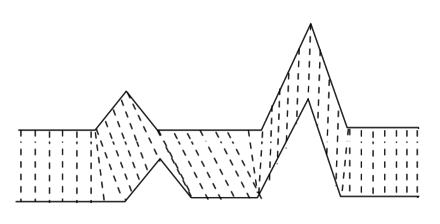
\includegraphics[width=8.5cm,height=5cm] {Dynamic_time_warping.png}
    \caption{Optimal map in Dynamic time warping, it allows the algorithm to
    find common learning patterns irrespective of point in time \cite{dtw_wiki}}
    \label{fig:dtwl}
\end{figure}

Having calculated the distances of all epochs, we now have to group them. For this, clustering seemed promising because there is not any early knowledge about classes. 
we considered hierarchical clustering approach of unsupervised learning where each observation starts in its own cluster, and pairs of clusters are merged as one moves up the hierarchy offering complete flexibility over the number of bins.

Once clusters are formed, we worked on appropriate visualization to present a given cluster for visual exploration.
Now to represent with multiple records within a cluster we look in direction of CDT.
We also take a look on other possible methods or concepts that could aid a more detailed perspective of model (Refer to figure .\ref{fig:flow_chart}).
we decided to use KNIME as a visualization tool to evaluate few methods on clusters.
The idea behind using a diversity of methods is to facilitate user with disparate visualizations to offer the possibility vivid perspective for the same data. For eg. while mean will represent the average weight, mode could be interesting when the user wants to know about the most common weight in a cluster. 

\begin{figure}
    \includegraphics[width=8.5cm,height=5cm] {Images/sorting/dtw_point.png}
    \caption{A combination of DTW, Agglomerative clustering and mean on weight data.
    Highlighted in red are the segments where weights show more fluctuations as compared to Weight Sum Sort in figure. \ref{fig:row_sum_epoch}}
    \label{fig:dtw_agl_mean}
\end{figure}
\subsubsection{Mean }
The most basic form for data summarizing and most susceptible to outliers, this quality of mean makes it useful to detect outliers weights. As shown in figure. \ref{fig:dtw_agl_mean} , the lines are more variation for same data, also there are fewer lines overlapping each other as compared to any prior visualization.

\subsubsection{Mode }
While it represents the most common weights amongst the bin, this offers us patterns representing more individual fluctuations in weights rather then averaging them.

\subsubsection{Median Absolute Deviation}
We already ruled out using the median as it loses the frequency information,  how about finding the deviation from median ? as it may help us find the diversion of data around a central point, this leads us to mean absolute deviation that comes from the area of statistical dispersion, where dispersion is (also called variability, scatter, or spread)  the extent to which a distribution is stretched or squeezed. Mean absolute deviation is a common method to measure the variability of a univariate sample of quantitative data.


\subsubsection{Regression, DTW and Agglomerative clustering}
\begin{figure*}
    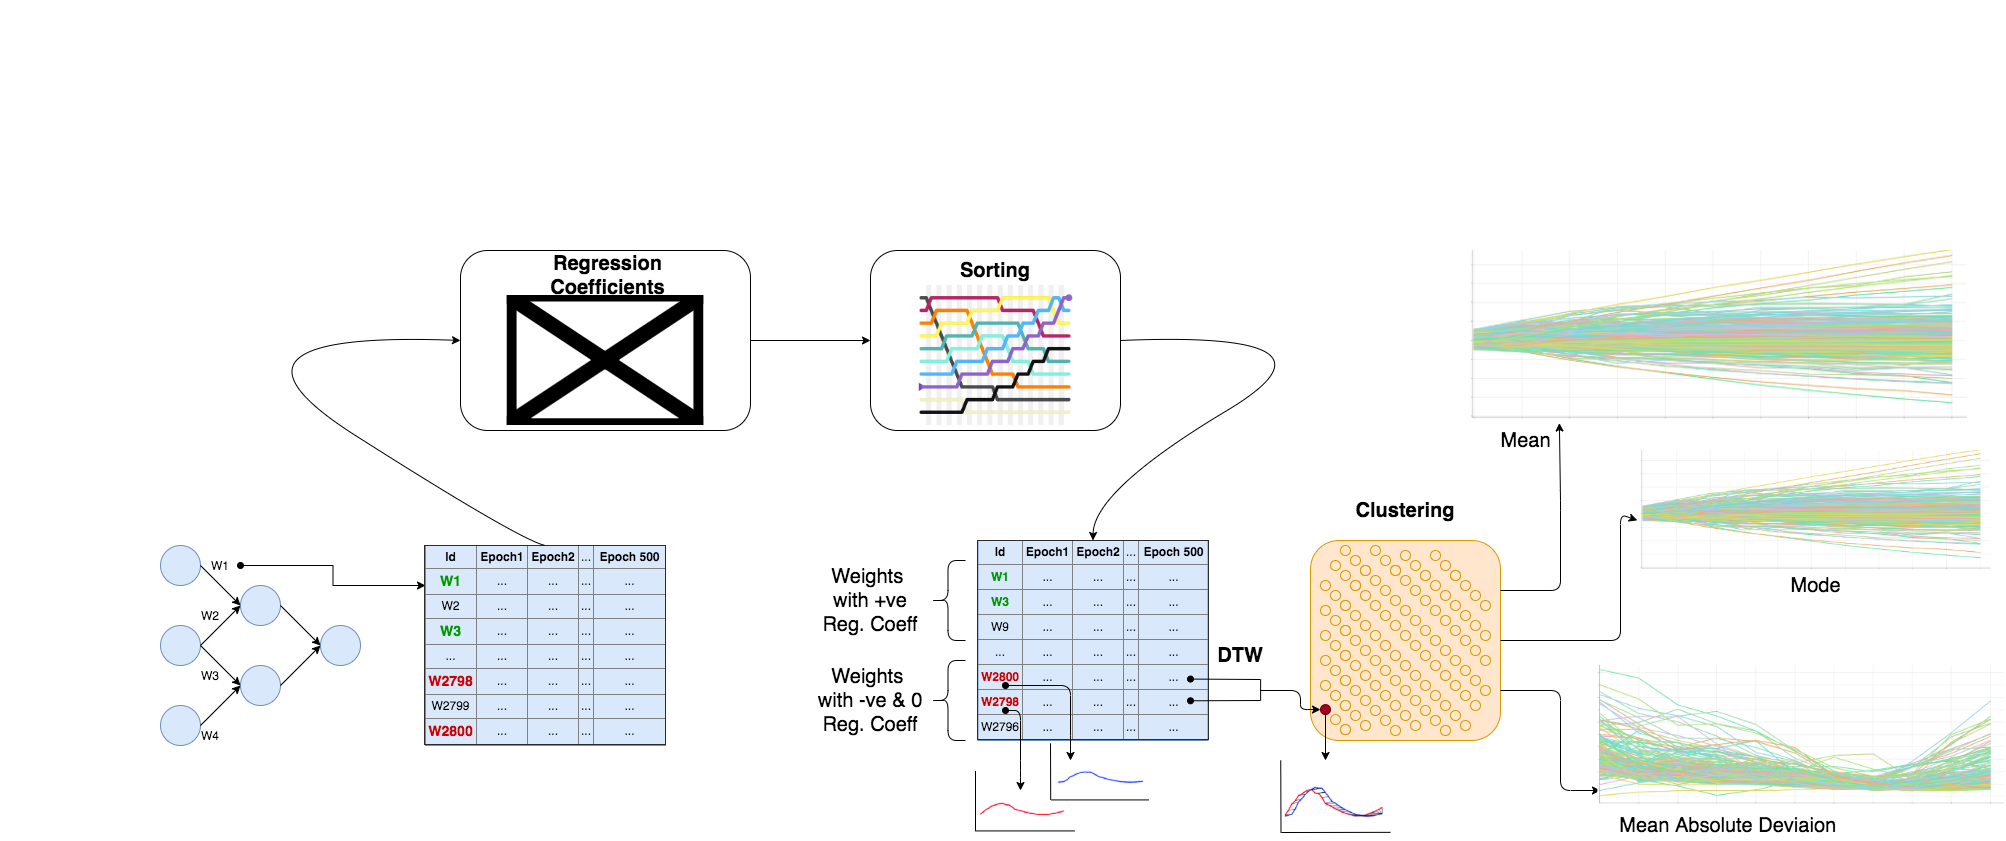
\includegraphics[scale=0.24]{Images/flow_chart.png}
    \caption{Flow chart explaining methods used in combination with DTW and agglomerative clustering.}
    \label{fig:flow_chart}
\end{figure*}



Undoubtedly, the combination of DTW and agglomerative clustering proved to be
of great use for our research but never the less, there is space for improvement.
considering same, we tried to juxtapose one typical method used in machine learning
i.e. linear regression (as shown in figure.\ref{fig:flow_chart}). In general, it's used as a method for ML but in this context, we are using it to further refine clusters by dividing the weights into 2 clusters based on their linear regression coefficient. 
We start with applying DTW on weights, the next step is to calculate
the regression coefficient of all training steps for each id. Once done, we divide the weights in a group of 2  based on the sign of the regression coefficient.
Post this we apply agglomerative clustering on each of the group. 
Once clustered, we visualized them individually as well as in combination.

As seen in figure.\ref{fig:reg_dtw_aggl} the lines reflect more sharper fluctuations in learning patterns.


\begin{figure}
    \includegraphics[width=8.5cm,height=5cm] {Images/sorting/dtw_reg_point.png}
    \caption{Regression grouping, DTW and Agglomerative clustering applied to weight data. The arrows point to area which is more spatially distributed as compared to visualization without Regression \ref{fig:dtw_agl_mean}}
    \label{fig:reg_dtw_aggl}
\end{figure}

\subsubsection{Breaking visualizations from model  to Layers}
Having worked multiple approaches to abstract the data.
we recognised that the visualization can be more interesting and useful if we break it down to even lower levels of model i.e layers.
This may be specifically useful for models where the number of Ids witnesses a drastic change from one layer to another as in that case the common weight of Ids 
is drastically different and presenting all on the chart comes with a trade-off for details. To achieve the same, we further altered the core of Tensorflow to yield layer-specific weights.
The visualization didn't just present with details as the chart was not formed to fit the range of just one layer's weights and the patterns which were otherwise suppressed to minuscule levels earlier now emerged more clearly and offered an even better data exploration.
%todo 

%mention about regression 
% work on this , does that rings bell that row sum and DTW has almost same lines with diff bin size , that automatically is a progress 

\subsection{Location tendency}
This determines the ”location” or shift of the distribution. We have used the concept of quantile to subdivide the weights of distribution into equal proportions. While the idea occurred naturally to sort data by our defined sorting methods and then divide them in quantiles but that eventually would have just been visualization to the statistical analysis of sorted Ids.
While in Location tendency, what matters is the value of data present at any given training step so we can completely forget Ids and sort data on every Epoch step to assign it to related quantile. The objective of this feature is to inform the user about the distribution of weight nearby zero, insights about this will further form base information for the possibility of model pruning (refer to figure \ref{fig:quantile}). We sailed through multiple approaches before finalizing, these were as follows  First Training Step  Sort,  Last Training Step Sort, Weight Sum Sort, Standard deviation sort and Individual training step sort. While all the above sorting methods claim to have some merits over the others, one common pattern followed by all is that they sort the data once and for all.
 The approach we used to calculate quantities is useful to analyse the overall weight distribution and also can be considered as a factor to determine the quality of model but can not be used as individual factors to get insights for pruning as the Ids are not taken into considering for this Viz.
 % add an image
 



\section{Utilizing Visualizations}
"Visualization gives you answers to questions you didn't know you had.” – Ben Schneiderman
This phrase exactly fits the scenario. We are trying to present data without having a complete idea of the use case that will be beneficial to the user. The overall goal is to present information in a balanced combination of high-level overview and detailed insights at the lower level.

Studying from a higher perspective, the most common reasons for bad accuracy \cite{ml_flaw1} \cite{ml_flaw2} are 
\begin{itemize}
\item Not enough training data 
\item Inappropriate activation function 
\item Too high or too low learning rate 
\item Inadequate training steps 
For a perfect visualization shall assist a user in ruling out some of the above possibilities if not point the exact one of the cause for a bad model.
\end{itemize}

To achieve the same, the visualization we developed offers the following features 
\begin{enumerate}
\item Visualize the timeline overview of the learning process of a model 
\item Can understand the central data tendency
\item Can avail "on-demand insights" 
\item Understand the distribution of weights 
\item Comprehend the spread of weights over time 
\item Perceive the range of weights over given training step
\end{enumerate}

Along with analysing the cause for bad accuracy, the above steps are the measures, if applied over a model with good accuracy, that may assist the user to the conclude whether or not to prune the weights and if yes, which and how many weights to prune with having least impact on accuracy.

% Defining the tasks that we want the  user to perform,  and then explaining the maths  and Viz methods used 




 


\section{Use Cases}
Here we present two cases to show how the workflow is represented in our system. First use case explicates the use of visualization for pruning while the other one facilities a developer who wants to enhance the efficiency of the model

\begin{figure}
    \includegraphics[width=8.5cm,height=5cm] {Images/UC1/uc1_quantile_pin.png}
    \caption{Lines showing the quantile division of weights in a model.}
    \label{fig:quantile}
\end{figure}
\subsection{Case 1} The first use case covers examining
the model for dead weighs.
In this scenario, the user is running a three layered dense model on MNIST\cite{mnist} data set.
He wants to reduce the processing time of the model by pruning dead weights.
To locate these weights, she/he analyses our method to comprehend location, distribution and learning pattern of weights .
Here is how she/he utilizes the available visualizations to assist his decision making.
\begin{enumerate}
\item Mean - This can give an initial estimate of the number of weights that are not learning. 
\item Location Tendency - With quantile visualization (figure \ref{fig:quantile}), the user registers that 3 quarters of weights lie in the interval of +0.2 to -0.2. She/He also learns that quantile 2 and quantile 3 lie in very close range of quantile 1. 
\item Standard Deviation -Based on the above insights, the user decides to filter set Sd filter criteria to 50 percent. This excludes 50 percent weights with least SD and presents the remaining weights.
\end{enumerate}
\begin{figure}
    \includegraphics[width=8.5cm,height=5cm] {Images/UC1/uc1_SD_filter.png}
    \caption{Lines presenting SD of clusters formed by combination of DTW and agglomerative clustering.}
    \label{fig:SD}
\end{figure}
On observing the SD chart (figure .\ref{fig:SD}) the user understands the learning degree of each cluster formed by DTW and agglomerative clustering. Relying upon his learning from visualizations, she/he decided the prune 25 a quarter of weights with least SD from the network.  
%TODO write the filter for SD in beter way 

\subsection{Case 2}
A physicist(AI expert) develops a ML model to classify the particle images from the microscope.
On the first run, she/he gets extremely low accuracy and validation accuracy. Our visualizations assist the user in exploring the insights further. Visualizing the weight sum sorting for the model (refer to the Fig. \ref{uc2_weight}), she/he infers 2 facts about the model i.e. 
 
 \begin{figure}
    \graphicspath{{\Images}}
    \includegraphics[width=8.5cm,height=5cm] {Images/UC2_5/usecase2_row_sum_failed_model.png}
    \caption{Weight Sum visualization of a ML model. The lines diverge initially but grows almost straight in end.}
    \label{uc2_weight}
\end{figure}


\begin{itemize}
\item Weights are diverging initially but are almost stable by the last training step 
\item The lines at the bottom of chart is showing different behaviour then rest of lines 
 \begin{figure}
    \includegraphics[width=8.5cm,height=5cm] {Images/UC2_5/usecase2_dtw_layer1.png}
    \caption{DTW and agglomerative clustering over weights for initial layer of a dense ML model.}
    \label{case2_dtw_layer0}
\end{figure}


% \item  Individual Layer DTW - As bins are more homogeneous now , the lines representing them are less smoother.

% %  \begin{figure}
% %     \includegraphics[width=8.5cm,height=5cm] {Images/UC2_5/dtw_layer1.png}
% %     \caption{Case 2 - DTW Layer 1}
% %     \label{case2_dtw_layer1}
% % \end{figure}


% %  \begin{figure}
% %     \includegraphics[width=8.5cm,height=5cm] {Images/UC2_5/dtw_layer2.png}
% %     \caption{Case 2 - DTW Layer 2}
% %     \label{case2_dtw_layer2}
% % \end{figure}


 

% \item Mode - It represents almost same shape as that of mean for give layer but just but less smooth due to even more alike weights. 
% \item Standard Deviation - Represent some parts of network are learning more then other 

\end{itemize}
While the first point rules out the possibility of a shortage of data or epochs the user suspects that second fact can be indicative of some crazy weights which are impacting the accuracy. To understand further, she/he decides to visualize the individual layer with DTW (Refer to fig 11) , agglomerative clustering and mode. After noticing that everything seems normal in all visualization, she/he concludes that inadequate data or training steps are not the reason for this accuracy and she/he then
continues his analysis further to check other reasons on his own.

\subsection{Case 3}An AI expert at airlines company runs an AI model to predict the seat occupancy for flights. The idea is to predict the seat occupancy using data of the first quarter of 2020 and based on that decide, the flight frequency to various destinations in upcoming months.
Compare to the results of the same model last year, the user witness a sharp decline in validation accuracy while accuracy is almost intact.Using our viz the user first observes DTW and agglomerative visualization  (refer to figure. \ref{case3_dtw_of}) for the model where she/he visualizes most of the lines to be almost straights which completely resembles less learning. Something that caught users attention is that there are some fluctuations in weights in initial epochs.
Which clearly reflects the following facts about model
\begin{figure}
    \includegraphics[width=8.5cm,height=5cm] {Images/UC3_2/UC3_of_layer1.png}
    \caption{Visualization of first layer weights of a ML model. The straight lines represent absence of learning in later learning steps.}
    \label{case3_dtw_of}
\end{figure}

\begin{itemize}
\item The training steps are optimal 
\item The model finds perfect weights which represent train data and this happened soon after the start
\end{itemize}
To further understand the model she/he views the DTW visualization for other layers which present almost same pattern.


\begin{figure}
    \includegraphics[width=8.5cm,height=5cm] {Images/UC3_2/UC3_per_layer1.png}
    \caption{Visualization of first later of same model as figure.\ref{case3_dtw_of}. This model is now trained on additional data. }
    \label{case3_dtw_layer0_fit}
\end{figure}


Concluding the above steps along with the simple loss landscape, the user decides to add more data to the training set and rerun the model. Now the model matches the validation accuracy expectations signing which the user wants again to visualize the new model to understand the cause of this change on visual grounds for which she/he sees a chart(figure. \ref{case3_dtw_layer0_fit}) that has barely any straight lines.



\section{Opportunities, Challenges and Discussions}

In this design study we researched various methods to study and analyse weights of ML models while we were able to come up with a useful visualization, but at this point, we have understood in detail the concepts of dynamic time analysis, limitations in binning of weights distribution, and have acquired knowledge about mathematical concepts that may be useful in this area. Our research also opens some gates to the following new opportunities for future work.
\begin{itemize}
\item Integrating our viz tool with Tensorboard - Tensorboard is a commonly used tool to visualize for machine learning experimentation. Integrating our visualization as a plugin to Tensorboard will make it handy to use. Hence, can benefit many ML experts with vital statistics about their models
\item Allowing changes in the model through GUI - Currently, user can only analyze the weight in our visualization. One important use case of this visualization is when a user uses this data to prune the model. An additional option to allow the user to prune the selected weights right away from GUI will thereby save the efforts of going to code and remove the weights manually. Further, rerun option may prove even more useful as a user can just perform everything in "exploration loop" \cite{knowGenMode} right from the GUI from analysing weights, pruning, rerunning and analysing the impact due to his changes.
\item Utilizing the layer hierarchy  - Data records often have some relationship to other pieces
of information \cite{keim2002information}. Right now we apply operations to weight without considering the impact of the weight of antecedent neurons. We can use this fact to further refine the process of binning. 
Let's take an example of the model as shown in fig:15, In the given case, the weights 46,47 and 56,57 appears to be have same values and learning at the same rate. All four will be considered the same for all our visualizations. While we completely ignore their dependence on preceding connections. In this case weight, 24 which forms in only connection of 46,47 is learning far more than 25 which indeed is responsible for weight 56,57. The idea here is to research these relations to seek possible impact over upcoming weights and this may prove an even better factor in binning the weights.


\end{itemize}
\begin{figure}
    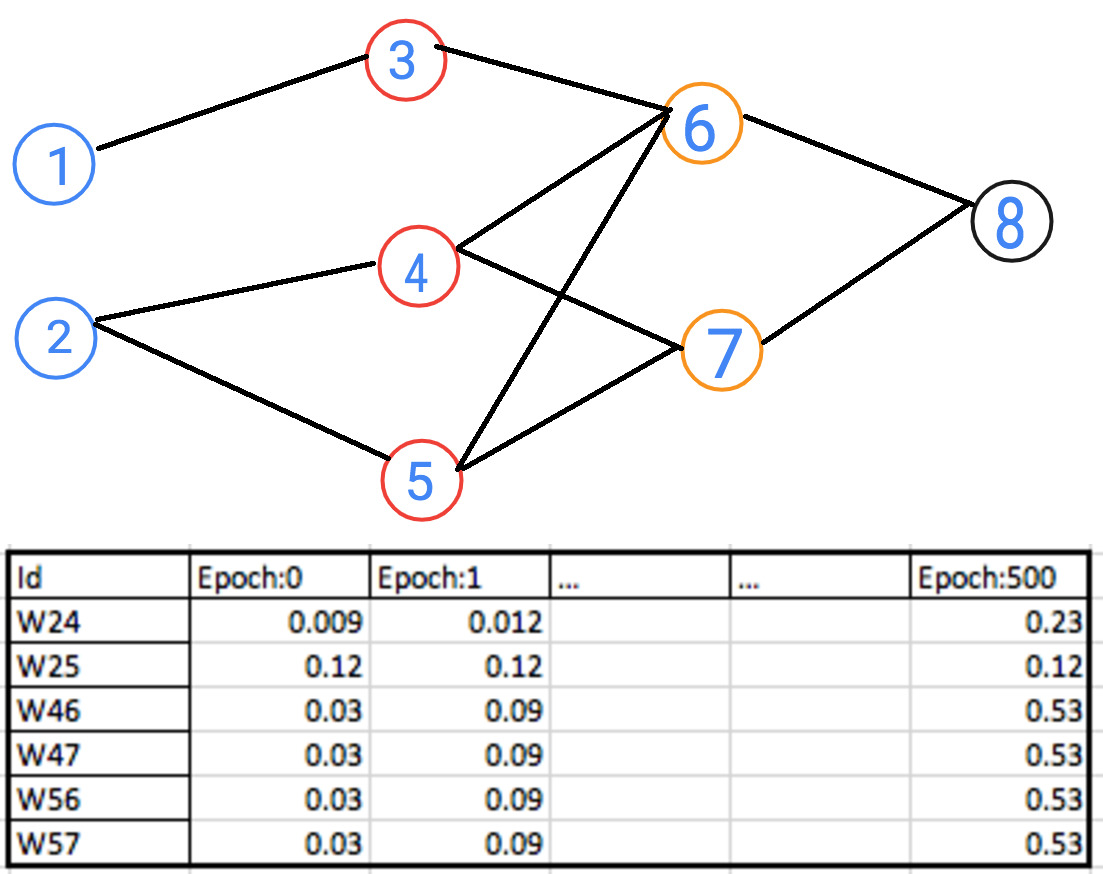
\includegraphics[width=8.5cm,height=5cm] {weight_rel.jpg}
    \caption{ Weights 46,47,48,49 will contribute equally to visualizations despite the variation in learning of their preceding Ids.}
    \label{weight_relations}
\end{figure}


During our research, we came across a question about the domain which we though to propose here in this section. We focused to produce a viz that is independent on all three factors determining a NN i.e Data, Domain and Model. Though we were able to achieve a platform that helps the user understand about weights and decide about the quality of the model. Many times during this time, we felt of using some concepts that completely explained the problem at hand but when we applied the same to other models/data sets, it made no sense at all. This left us with very limited options to choose from. While making those trade offs, we felt, if is it really plausible to think of a model that servers all ML models, data and domains or this will end up with insights too assorted and generic that user may not find it enough interesting.


\section{Conclusion}
We started with analysing the existing XAI methods and their dependencies.
Post that, we ponder upon intrinsic features of ML models 
which we can use as a foundation for XAI method.
This was followed by presenting ways to sort and bin data. 
Research also lead us to  development of new criteria for sorting i.e. weight sum sort which proved a step above traditional sorting methods.
Apart from standard methods, we introduce the utility  of 
Dynamic time warping, agglomerative clustering and their combination with regression 
for analysing patterns of learning.
Besides the methods, we also customize the tensor flow to produce weight files for individual layers 
which provided us with a more detailed perspective.
We used Knime and D3  to create a visualization that offers the user control over bin count, clustering method and sorting method. 
The interactive zoom and quantiles were designed specifically to make sure that the user has both upper and lower level views available.
Use cases presented the description of how our method can be used to determine the quality of machine learning model
in a meaningful way that empowers an ML expert to run plug and play analysis for the model without 
having to go through time taking configuration process. 
At last, we mentioned the questions that we couldn't answer and carries potential 
to prove a big leap in direction generalizing XAI.

\bibliographystyle{abbrv}
%%use following if all content of bibtex file should be shown
%\nocite{*}
\bibliography{template}


\end{document}
